\chapter{Introduction} \label{Introduction}

Systems that work in a repetitive manner, such as robotic manipulators and chemical plants, use Iterative Learning Control (ILC) to iteratively improve the performance over a given repeated task or trajectory. The feed-forward control signal is modified in each iteration to reduce the error or the deviation from the given reference trajectory. A good analogy is a basketball player shooting a free throw from a fixed position: during each shot the basketball player can observe the trajectory of the ball and alter the shooting motion in the next attempt \cite{Survey}. 

The limitation with ILC is that it assumes the task or the trajectory to be fixed (constant) over iterations. While this is a reasonable assumption to make in some repeated tasks, ILC cannot handle the cases when the trajectory is modified or changing over time, and the learning controller must start learning from scratch. It is shown in this thesis that a significant amount of knowledge can be transferred even between cases where the reference trajectories are not the same. A basketball player does not have to learn the free throw motion from scratch each time he finds himself in a slightly different position. We call these different cases or reference trajectories \textit{contexts}. Context can change in a given task and it is the responsibility of the autonomous agent or the learning controller to adapt to different contexts. 

The motivation for transfer learning under different contexts comes mainly from the RoboEarth project \cite{RoboEarth}, a robot specific knowledge repository where robots share and learn from each others' experience.  The ability to transfer knowledge even under different contexts will significantly improve the performance of RoboEarth.  As an example, consider a robot operating in a private home in Eindhoven learning to pour tea from a teapot into a teacup, and over time perfecting the motion. The learned pouring motion can be uploaded to RoboEarth, marked with the hardware-specifics of the particular robot as well as the size and shape of the teapot/teacup as context. Another robot in Zaragoza \footnote{University of Zaragoza and Eindhoven University of Technology are partners with ETH Z\" urich in the RoboEarth project. For the list of all partners and other details visit http://www.roboearth.org/} 
with slightly different hardware and holding a different teapot, can download the stored motion as a prior and adapt it to its particular context, thereby eliminating the need to learn the motion from scratch. 

\section{Gaussian Processes}\label{GPIntro}
To accomplish this type of task we have used Gaussian Processes for cost function prediction and knowledge transfer between different contexts. A \textit{Gaussian Process} (GP) is a collection of dependent random variables, any finite number of which have a joint Gaussian distribution \cite{GPbook}. 

Gaussian processes, completely specified by a mean function $\mu(x)$ and a covariance (or kernel) function $k(x,x')$, can be seen as a prior distribution over the space of functions. For $y_i = f(x_i) + \epsilon_i$, $\epsilon_i \sim \mathcal{N}(0,\sigma_{n}^{2})$ with noisy observations $\observations_{N} = \{y_1,\ldots,y_N\}$ at sample points $X = \{x_1,\ldots,x_N\}$, the posterior over $f$ is again a Gaussian Process distribution with mean $\mu_N{(x)}$ and covariance $k_N(x,x')$ given by the following simple analytic equations:

\begin{align}
\mu_N{(x)} = \mu(x) + \mathbf{k}_N(x)^{\mathrm{T}}[\mathbf{K}_N + \sigma_{n}^{2}\mathbf{I}]^{-1}(\observations_N - \boldsymbol{\mu}_N) \label{gpUpdate_mu} \\ 
k_N(x,x') = k(x,x') - \mathbf{k}_N(x)^{\mathrm{T}}[\mathbf{K}_N + \sigma_{n}^{2}\mathbf{I}]^{-1} \mathbf{k}_N(x') \label{gpUpdate_sigma}
\end{align}

where $\boldsymbol{\mu}_N = [\mu(x_1),\ldots,\mu(x_N)]^\mathrm{T}$ is the prior mean at the sample points,  \\ $\mathbf{k}_N(x) = [k(x_1,x),\ldots,k(x_N,x)]^\mathrm{T}$ is the vector of covariances at the same points and $\mathbf{K}_N = [k(x,x')]_{x,x' \in X} \succeq 0.$

The mean update equation (\ref{gpUpdate_mu}) is a linear predictor because the resulting mean $\mu_N{(x)}$ is a linear combination of noisy observations $\observations$. 	

In the covariance update equation (\ref{gpUpdate_sigma}) the quantity $\mathbf{k}_N(x)^{\mathrm{T}}[\mathbf{K}_N + \sigma^{2}\mathbf{I}]^{-1} \mathbf{k}_N(x')$ corresponds to the \emph{information gain} from the noisy observations, i.e. reduction in uncertainty from the prior covariance $k(x,x')$.

With these update equations, Gaussian processes can be used in nonparametric regression to predict the mean and variance of unknown test points. Nonparametric regression methods have the advantage of avoiding overfitting issues encountered typically in regression with finite basis functions. The prior models specified by the mean and variance functions, chosen among a discrete set of possible model structures  $\mathit{H_i}$ (including composites) usually have a lot of flexibility. They can be further optimized by optimizing \textit{hyperparameters} using likelihood functions for training data. The likelihood function specifies the probability of the noisy training data $\observations$ given the sample points $X = \{x_1,\ldots,x_N\}$ and the latent function $f$, drawn from a GP with corresponding hyperparameters. See Chapter \ref{Chapter2} for details on hyperparameter estimation and likelihood functions.

Gaussian processes have been used in the statistics community for a long time, especially in geostatistics, where the update equations  (\ref{gpUpdate_mu}) and (\ref{gpUpdate_sigma}) are known under the name \textit{kriging}. Geostatistics has traditionally confined \textit{kriging} to 2-dimensional and 3-dimensional spatial modelling problems. However, GP is currently applied extensively in machine learning, mostly in Bayesian supervised learning, in high-dimensional regression and classification problems.
% ref needed?

Gaussian Processes when used in estimation, have the advantage of capturing the entire distribution over future values of the function instead of merely their expectation \cite{Rasmussen2}, but unlike Kalman filters require $O(N^3)$ complexity due to the prohibitive matrix inversion in (\ref{gpUpdate_mu}) and (\ref{gpUpdate_sigma}). 
Several reduced-rank approximations are reported in the literature \cite{GPbook} to overcome the problem of growing $N$ especially in big datasets.
%

\section{Contextual Bandits}
\label{ContextBandit}

Multi-armed bandit problems is the basic setting in decision theory and reinforcement learning to optimally balance \textit{exploration} and \textit{exploitation}. In the context of stochastic function optimization, in order to find the global minimum of an unknown noisy function, it must be \textit{explored} by sampling at promising points and must be \textit{exploited} at the current minimum values. Using upper confidence bounds (UCB) is a particularly simple and intuitive heuristic to balance the exploration/exploitation trade off and works by keeping track of upper confidence bounds of the sample points \cite{Krause1}. When applied to dynamical systems, the sample points are the control signals and the function to be minimized is the cost function. Although the cost function with respect to the system output is well defined, the cost corresponding to the control signal is not completely known due to modeling errors and unknown external disturbances. Therefore, multi-armed bandits can be used to track the global minimum of this cost function while providing a framework that can be extended for knowledge transfer.

In addition to the controller input, contexts such as the current internal state of the system, the current environment state, and desired state can be parameterized in the cost function. 
Learning over the joint space of inputs and contexts enables the knowledge transfer between different learning controllers with different contexts. 
With the addition of context, bandit problems transform into a full-scale reinforcement learning problem \cite{sutton98a}. In reinforcement learning literature, tracking the global optimum is known as minimizing the cumulative regret $R_{T} = \Sigma_{t = 1}^{T}r_{t} $ or equivalently maximizing the cumulative reward (the negative of cumulative regret). Here $r_{t}$ is the instantaneous regret $r_{t} = f(x_{t}) - f(x^{*})$, $x^{*} = \operatorname*{arg\,min}_{x \in \mathit{D}}f(x)$. 

A desired feature of a (reinforcement) learning algorithm is to have sublinear regret because then the average regret $R_{T}/T$ after T rounds will be bounded. This means the algorithm will be converging to the optimal action over time, with convergence rate depending on the sublinearity. Krause et al. in \cite{Krause2}, discuss such a learning algorithm (called CGP-UCB) which maintains a GP-estimate of the function to be optimized: 
\begin{equation}
\sysInput_{t} = \operatorname*{arg\,min}_{\sysInput \in U}\mu_{t-1}(\sysInput;\context_t) - \beta_{t}^{1/2}\sigma_{t-1}(\sysInput;\context_t) \label{ucb}
\end{equation}

where $\mu_{t-1}$ and $\sigma_{t-1}$ are the posterior mean and standard deviation of the GP over the joint input-context space $U \times C$, conditioned on the observations $(\sysInput_1,\context_1; y_1),\ldots,(\sysInput_{t-1},\context_{t-1}; y_{t-1})$ and $\beta_{t}$ is the confidence parameter that scales exploration vs. exploitation for the particular problem. Thus, when presented with context $\context_t$, this algorithm uses GP-inference in (\ref{gpUpdate_mu}) and (\ref{gpUpdate_sigma}) to predict mean and variance for each possible action $\sysInput$, conditioned on all past observations.

Regret bounds always hold with probability $1-\delta$ only, since they're derived from probabilistic inequalities. More concretely, it is the result of two factors:

1. If a function is drawn from a GP with mean $\mu(x)$ and covariance $k(x,x')$, variance $\sigma^{2}(x) = k(x,x)$, the following bound on the function holds with probability $ \geq 	1 - \delta$, where $\delta$ is a suitably chosen value, $0 < \delta \leq 1$ determining the value of the confidence parameter $\beta$:

\begin{equation}
|f(x) - \mu_{t-1}(x)| \leq \beta_{t}^{1/2}\sigma_{t-1}(x) \qquad \forall x \in D, \forall t \geq 1
\label{function bound}
\end{equation}

For functions belonging to the Reproducing Kernel Hilbert Space (RHKS) of $k(x,x')$, the bound is essentially the same:

\begin{equation}
Pr \big\{ \forall T, ||\mu_{T} - f||_{k_{T}}^{2} \leq \beta_{T+1} \big\} \geq 1 - \delta
\end{equation}

2. To show sublinear regret for a finite number of trials $T$, where $x_{T}$ are chosen, it is necessary that the function to be optimized obeys some sort of a regularity condition, ensuring smoothness at least probabilistically. In this case the kernel structure $k(x,x')$ plays a big role. Functions drawn from such a kernel must satisfy the following Lipschitz-like bound:

\begin{equation}
Pr \big\{ \sup_{x \in D} |\partial f/\partial x_{j}| \geq L \big\} \leq a e^{-(L/b)^{2}}, j = 1, \ldots, d
\label{Lipschitz-like bound}
\end{equation}

where, $a,b$ are some constants, and $d$ is the dimension of $x$. 

Sample paths of functions drawn from a GP with mean $\mu(x)$ and kernel $k(x,x')$ are rougher than RHKS functions with the same defined kernel. For such RHKS functions, assumption (\ref{Lipschitz-like bound}) is not necessary.

\subsection*{Test Case}
% Add 2 figures showing decrease in uncertainty after picking a point

Here we show learning results for a one-dimensional test case where we generate 50 functions drawn from a Gaussian process with squared exponential kernel. For hyperparameter values, the length-scale parameter $l = 0.1$, the scale parameter $\sigma_{s}^{2} = 1$ and the noise variance $\sigma_{n}^{2} = 0.025$. Cholesky decomposition of the covariance matrix has been used to generate the functions, and a small $\epsilon = 0.003$ value has been added to the diagonals of the covariance matrix to prevent singularity issues often complicating the use of the squared exponential kernel. This effect can be seen in Figure \ref{fig:func}, where the first 10 functions sampled from the GP are shown. 

Non-contextual GP optimization can be seen in Figures \ref{fig:gpucb1} and \ref{fig:gpucb2}. At each time stage, the algorithm is picking the point $x$, labeled with the plus sign, that minimizes $\mu_{t-1}(x) - \beta_{t}^{1/2}\sigma_{t-1}(x)$. The figures show the decrease in uncertainty after picking a point. The uncertainty at the sampled point reduces to the standard deviation of the noise, $\sigma_{n}$.

\begin{figure}
\center
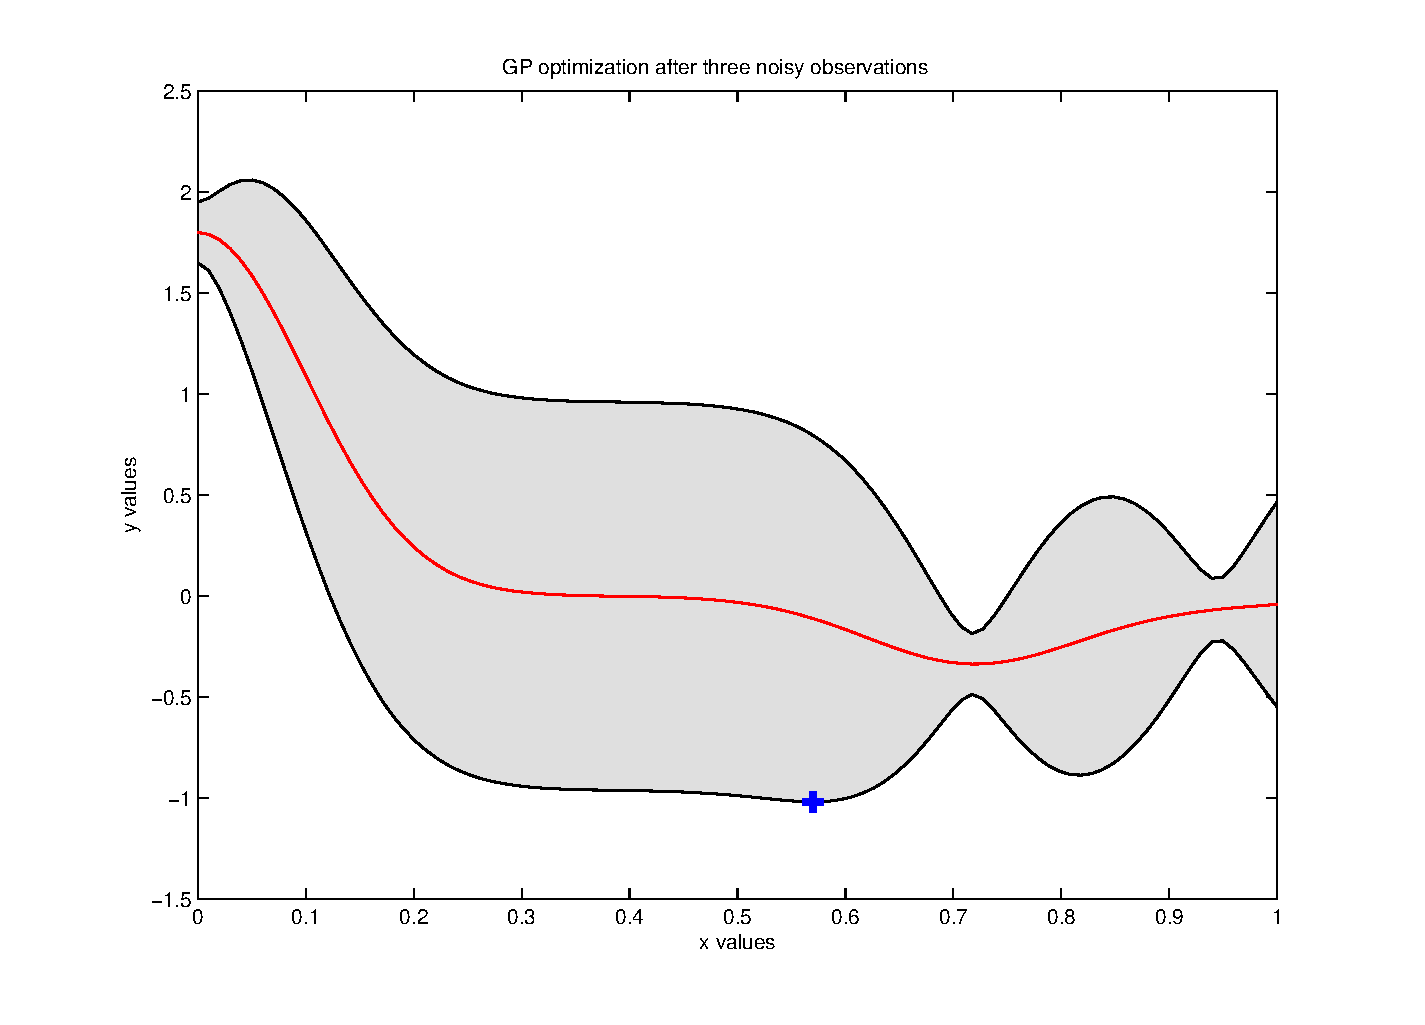
\includegraphics[scale=0.40]{test_gpucb1.eps}			
\caption{GPUCB optimization at time step 4}
\label{fig:gpucb1}
\end{figure}

\begin{figure}
\center
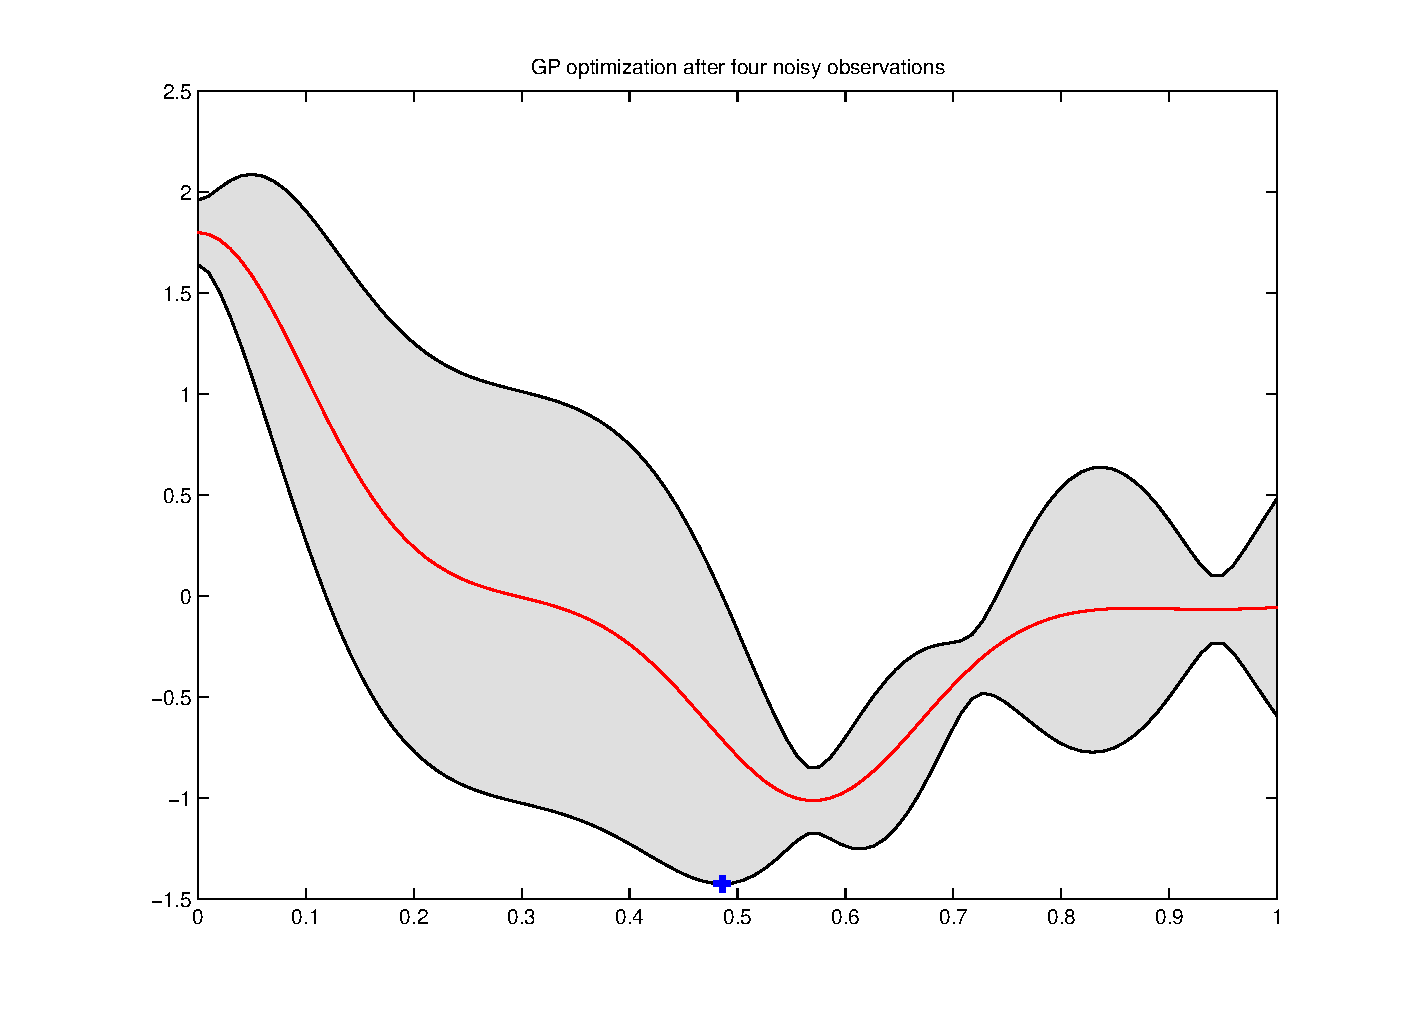
\includegraphics[scale=0.40]{test_gpucb2.eps}			
\caption{GPUCB optimization at time step 5}
\label{fig:gpucb2}
\end{figure}

The cumulative regret shown in Figure \ref{fig:cumregret} is averaged over 50 trials. For the $\beta_{t}$ value, Theorem 2 has been used, but it has been scaled down by 20. That is:

\begin{equation}
\beta_{t} = \frac{2 \log(t^{2}2 \pi^{2}/(3\delta)) + 2d\log(t^{2}dbr\sqrt{\log(4da/\delta)})}{20} \label{Thm2KrauseBeta}
\end{equation}

where $a = 1, b = 1, d = 1, r = 1$ and $\delta = 0.1$. 

\begin{figure}[h!t]
\center
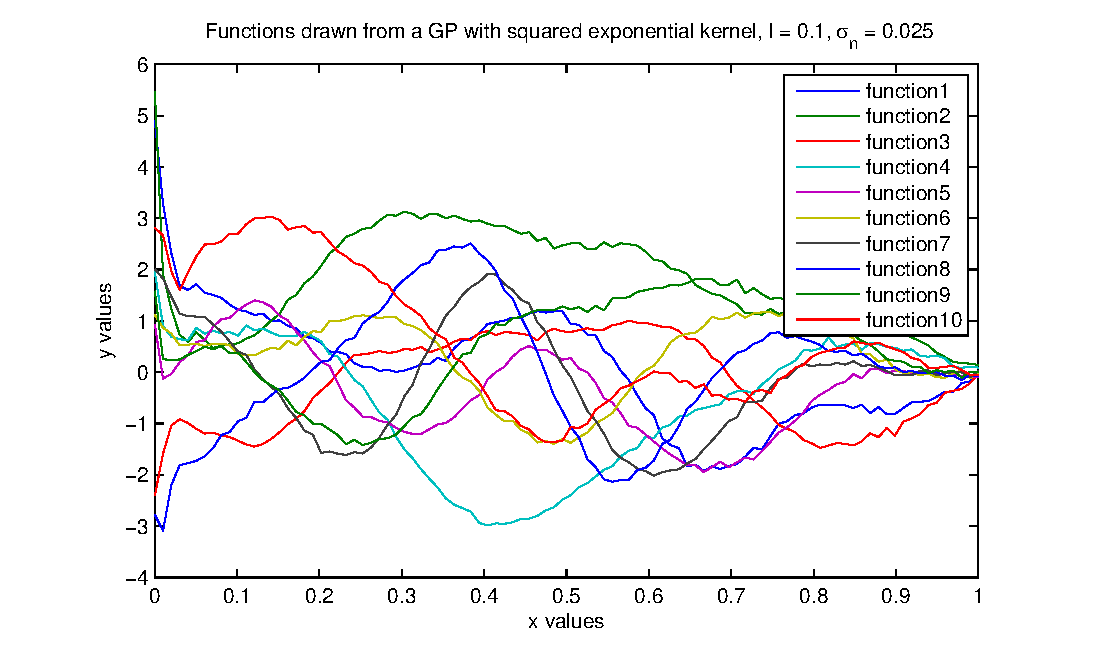
\includegraphics[scale=0.50]{functions.eps}			
\caption{Functions sampled from a Gaussian Process}
\label{fig:func}
\end{figure}

\begin{figure}[h!t]
\center
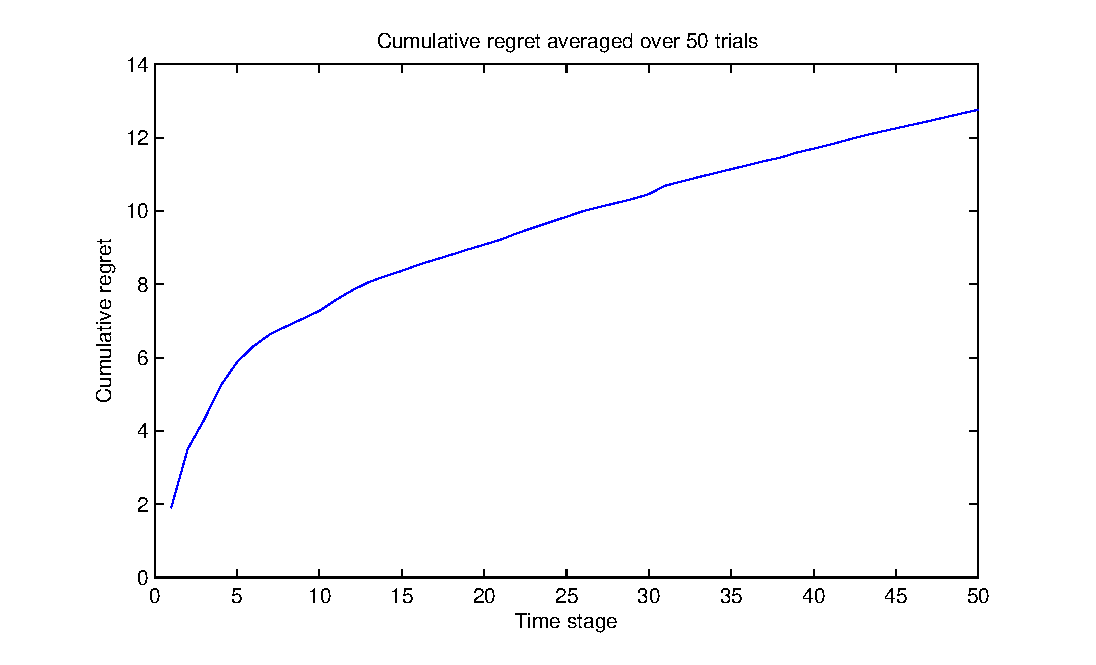
\includegraphics[scale=0.50]{test_cumregret.eps}			
\caption{Cumulative regret averaged over 50 trials}
\label{fig:cumregret}
\end{figure}

The shape of the cumulative regret growth agrees with the theoretical $\mathcal{O}(T^{1/2})$ growth. 

\section{Related Work}

Gaussian Processes are increasingly applied in control, where they are used to learn the unknown system dynamics. In \cite{Blimp} the authors propose a hybrid-GP approach combined with reinforcement learning to control an autonomous blimp. 
This approach closely parallels that of ours, the main differences lie in the use of the scalar cost function and the CGP-UCB framework, as will be detailed in the next sections. Their framework requires them to model the dynamics itself with a GP, and this is computationally very prohibitive as the number of dimensions increase. In \cite{PILCO,Deisenroth} the authors first learn the dynamics with GP. In the second step policies for a parameterized controller are learnt by propagating through the GP model. This method involves necessarily long offline calculations and many repeated trials. The method proposed in this paper aims to learn at every stage by incorporating feedback, and learns \emph{only} the stage cost, as a function of input and context, as opposed to the whole dynamics.

Gaussian process optimization literature proposes several heuristics such as Expected Improvement \cite{Jones01ataxonomy} and Most Probable Improvement \cite{Lizotte07automaticgait} for trading off exploration and exploitation. The first method with provable sublinear regret was proposed in \cite{Krause1}. The results of \cite{Krause1} were extended to the contextual setting in \cite{Krause2}, which is applied to dynamical systems in this thesis.
